%-----------------------------------------------------------------------------
%
%               Template for sigplanconf LaTeX Class
%
% Name:         sigplanconf-template.tex
%
% Purpose:      A template for sigplanconf.cls, which is a LaTeX 2e class
%               file for SIGPLAN conference proceedings.
%
% Guide:        Refer to "Author's Guide to the ACM SIGPLAN Class,"
%               sigplanconf-guide.pdf
%
% Author:       Paul C. Anagnostopoulos
%               Windfall Software
%               978 371-2316
%               paul@windfall.com
%
% Created:      15 February 2005
%
%-----------------------------------------------------------------------------


%% \documentclass{sigplanconf}
%% \documentclass[preprint]{sigplanconf}
\documentclass[preprint, 10pt]{sigplanconf}

% The following \documentclass options may be useful:

% preprint      Remove this option only once the paper is in final form.
% 10pt          To set in 10-point type instead of 9-point.
% 11pt          To set in 11-point type instead of 9-point.
% numbers       To obtain numeric citation style instead of author/year.

\usepackage{amsmath}
\usepackage{graphicx}
\usepackage{hyperref}
\usepackage{booktabs}
\usepackage{listings}

\hypersetup{
  colorlinks=true,
  linkcolor=blue,
  citecolor=blue
}

\lstset{
  basicstyle=\footnotesize,
  numbers=left
}

\newcommand{\cL}{{\cal L}}

\begin{document}

\special{papersize=8.5in,11in}
\setlength{\pdfpageheight}{\paperheight}
\setlength{\pdfpagewidth}{\paperwidth}

\conferenceinfo{CONF 'yy}{Month d--d, 20yy, City, ST, Country}
\copyrightyear{20yy}
\copyrightdata{978-1-nnnn-nnnn-n/yy/mm}
\copyrightdoi{nnnnnnn.nnnnnnn}

% Uncomment the publication rights you want to use.
%\publicationrights{transferred}
%\publicationrights{licensed}     % this is the default
%\publicationrights{author-pays}

% These are ignored unless 'preprint' option specified.
\titlebanner{DRAFT}
\preprintfooter{DRAFT --- Nash: a tracing JIT for GNU Guile}

\title{Nash: A Tracing JIT VM For GNU Guile}
%% \subtitle{Subtitle Text, if any}

\authorinfo{Atsuro Hoshino}
           {Individual Software Developer}
           {hoshinoatsuro@gmail.com}
%% \authorinfo{Name2\and Name3}
%%            {Affiliation2/3}
%%            {Email2/3}

\maketitle

\begin{abstract}

This paper introduces \textit{Nash}, a \textit{virtual machine} (VM) for GNU
Guile with tracing \textit{just-in-time} (JIT) compiler. When conditions were
met, Nash runs \textit{$40\times$ faster} than Guile's existing VM, without
modifying the input program source code. Benchmarks have shown performance close
to other Scheme implementations which compile to native code.

Design of Nash internal is discussed. Nash coexists with Guile's existing VM,
uses the existing VM during native code compilation. Lots of Guile's features,
such as bytecode compiler, bytecode interpreter, are reused in Nash. Nash could
be used as a drop-in replacement of Guile's existing VM.\@ Guile contains
bytecode compiler, which is designed as a compilation tower. The compiler tower
design enables compiling and running other language than Scheme, which means
that Nash could be used as a VM for other languages.
\end{abstract}

%% \category{CR-number}{subcategory}{third-level}

% general terms are not compulsory anymore,
% you may leave them out
%% \terms
%% term1, term2

\keywords{} Scheme~Programming~Language, Just-In-Time~Compiler, Virtual~Machine,
Implementation,

\section{Introduction}

From its simple design, Scheme is used for various purposes, many
implementations exist. One of the use is as an extension language embedded in
other program. Implementations such as Chibi-Scheme, TinyScheme are suited for
use as an extension language. Another use is for scripting. Scheme
implementations for scripting typically have fast start up time, and features
for daily programming tasks. Gauch, for instance, is designed to suite the use
for scripting. Scheme implementation such as Ypsilon is designed for real-time
application. On the other hand, there are Scheme implementations used for more
expensive computation than scripting. This kind of Scheme implementations
typically compiles to native code before executing. The compilation could be
done \textit{ahead-of-time} (AOT), such as in Bigloo~\cite{serrano1995bigloo}
and Gambit~\cite{feeley1998gambit}, or incrementally, such as in
Chez~\cite{dybvig2006development} and Larceny~\cite{hansen1992impact}, or in a
mixture of AOT bytecode and JIT compilation, such as in
Pycket~\cite{bauman2015pycket}, and Racket~\cite{flatt2013racket}.

There exist a performance gap between Scheme implementations doing native code
compilation, with implementations do not. Tracing JIT compilation is a
technique used in VM to improve performance by compiling the frequently
executed instructions in loops. Dynamo~\cite{bala2000dynamo} has pioneered the
use of tracing JIT by tracing native code. Later the technique was used in
various VMs for dynamic programming language to achieve performance
improvement. Languages such as Lua~\cite{pall2016luajit},
JavaScript~\cite{gal2009trace}, and Python~\cite{bolz2009tracing} have made
success with VMs which implements tracing JIT.\@

\textit{Nash} is a new tracing JIT VM for GNU Guile. Guile is a
general-purpose Scheme implementation which could be used as an extension
language, as a scripting engine, and for application development. Guile offers
\textit{libguile} to allow itself to be embedded in other program. GnuCash,
gEDA, GNU Make, and GDB uses Guile as an extension language. Guile implements
standard R5RS~\cite{abelson1998revised5}, most of
R6RS~\cite{sperber2010revised}, several SRFIs, and many extension of its own,
including delimited continuation and native POSIX thread
support~\cite{Galassi02guilereference}. Nash is designed as a drop-in
replacement for Guile's existing VM, which is called \textit{VM-regular} in
this paper, to achieve performance improvement.

\begin{figure}
  \begin{center}
    \small
\begin{verbatim}
1 (define (sample-sum vec)
2   (let lp ((i 0) (acc 0))
3     (if (<= (vector-length vec) i)
4         acc
5         (lp (+ i 1)
6             (if (< 0 (vector-ref vec i))
7                 (+ acc (vector-ref vec i))
8                 acc)))))
\end{verbatim}
\end{center}
\caption{Scheme source code of sample procedure.}
\label{fig:scmloop}
\end{figure}

Figure~\hyperref[fig:scmloop]{\ref{fig:scmloop}} shows Scheme source code of a
sample procedure \texttt{sample-sum} which contains a loop. The procedure
takes a single argument \texttt{vec}, a vector containing numbers. The loop
inside \texttt{sample-sum} checks whether the \texttt{i}-th
\texttt{vector-ref} of \texttt{vec} is greater than \texttt{0}, adds up the
element if true. The loop repeat the comparison and addition with incremented
\texttt{i} until \texttt{i} is greater than the \texttt{vector-length} of
\texttt{vec}. In Guile, Scheme source codes are compiled to bytecode before
the execution.\footnote{In most case, source codes are byte-compiled before
  executed. Guile can run Scheme source code without compiling so that trivial
  computations could be done quickly.}
Section~\hyperref[sec:background]{\ref{sec:background}} briefly mentions how
existing bytecode compiler in Guile works. When Nash execute
\texttt{sample-sum}, the computation starts with bytecode interpreter. After
executing the bytecode for a while, the bytecode interpreter detects a hot
loop in the body of \texttt{sample-sum} (from line 2 to line 8 in
Figure~\hyperref[fig:scmloop]{\ref{fig:scmloop}}). Then the bytecode
interpreter switches its state, start recording the bytecode instructions of
the loop and values in the stack. Recording traces are described in
Section~\hyperref[sec:interpreter]{\ref{sec:interpreter}}. When the bytecode
interpreter reached to the beginning of the observed loop, bytecode the
recorded traces are passed to a JIT compiler. The JIT compiler is written in
Scheme, executed by VM-regular. The compiler uses recorded bytecode and stack
values to emit optimized native code. The variables from the stack are used to
specify types, possibly emitting \textit{guards} to exit from the compiled
native code. Details of the JIT compiler is covered in
Section~\hyperref[sec:compiler]{\ref{sec:compiler}}. The details of Nash
internal are explained with using \texttt{sample-sum}.

The rest of the sections are organized as follows.
Section~\hyperref[sec:evaluation]{\ref{sec:evaluation}} shows results from
benchmark, including comparisons between Nash and other Scheme
implementations. Section~\hyperref[sec:related]{\ref{sec:related}} mentions
related works. Finally, Section~\hyperref[sec:conclusion]{\ref{sec:future}}
discusses possibilities for future work, and
Section~\hyperref[sec:conclusion]{\ref{sec:conclusion}} concludes this paper.

\section{Background}
\label{sec:background}

This section describes background information and brief history of tracing JIT
and GNU Guile. Some of the Guile internals which relates to Nash are
mentioned.

\subsection{Tracing JIT}
Tracing JIT is one of JIT compilation style~\cite{bolz2009tracing} which
assumes that:

\begin{itemize}
\item Programs spend most of their runtime in loops.
\item Several iterations of the same loop are likely to take similar code
  paths.
\end{itemize}

After Dynamo~\cite{bala2000dynamo} used the technique to trace native code,
various development has been done in the area. LuaJIT is one of the successive
implementation of tracing JIT VM for the Lua~\cite{ierusalimschy1996lua}
programming language. Pypy~\cite{bolz2009tracing} is a tracing JIT VM for the
Python programming language. Pypy is implemented with using
RPython~\cite{bolz2009tracing} framework, which is a \textit{meta-tracing}
infrastructure to develop a tracing JIT VM by defining a interpreter of the
target language. The framework was adapted to other language than Python,
including Pycket~\citep{bauman2015pycket}, a tracing JIT VM for Racket
language, and Pixie, a tracing JIT VM for Pixie language, which is a dialect
of Lisp.

Typical settings for tracing JIT of dynamic programming language contains an
interpreter and a JIT compiler. Interpreter observes the execution of bytecode,
detects hot loops, and records frequently executed instructions. The recorded
instructions are often called as \textit{trace}. JIT compiler then compiles the
trace to get optimized native code of the hot loop. The interpreter typically
has a functionality to switch between a phase for observing the loop, a phase
for recording the instructions, and a phase executing the compiled native code.
Compiled native code contains \textit{guards} to terminate the execution of
native code, and bring the control of program back to the interpreter. Guards
are inserted when recorded trace contains conditions which might not satisfied
in later iterations of the loop. For instance, the loop in
Figure~\hyperref[fig:scmloop]{\ref{fig:scmloop}} will emit a guard which
compares the value of \texttt{i} with length of the vector. In dynamic
programming language such as Scheme, guard for type check may inserted as well,
since compiler could generate more optimized native code when the types of the
values are known at compilation time.

\subsection{GNU Guile}
\label{sec:backgroundguile}

GNU Guile was born to be an official extension language for GNU
projects~\cite{Galassi02guilereference}. Since then, various developers have
made changes to the implementation. As of version 2.1.2, Guile contains a
bytecode compiler, and a VM which interprets bytecode. Guile uses conservative
Boehm-Demers-Weiser garbage collector~\cite{boehm1988garbage}.

% Might worth mentioning libguile again.

\subsubsection{SCM Data Type}
\label{sec:scmdatatype}

\begin{table}
  \begin{center}
  \begin{tabular}{ccl}
    \toprule
    Tag&Type&Scheme value\\
    \midrule
    \texttt{XXXXXXXXXXXXX000} & heap object & `foo, \#(1 2 3) \ldots \\
    \texttt{XXXXXXXXXXXXXX10} & small integer & 1, 2, 3, 4, 5 \ldots \\
    \texttt{XXXXXXXXXXXXX100} & boolean false & \#f \\
    \texttt{XXXXXXXX00001100} & character & \#\textbackslash{} a,
    \#\textbackslash{} b, \ldots \\
    \texttt{XXXXXX1100000100} & empty list & `() \\
    \texttt{XXXXX10000000100} & boolean true & \#t \\
    \bottomrule
  \end{tabular}
  \end{center}
  \caption{Tag value with corresponding Scheme type and Scheme value. The
    ``\texttt{X}'' in the tag column indicates any value.}
\label{tab:tags}
\end{table}

From the need of being an extension language, Guile's internal data type is
defined as typedef \texttt{SCM} in
C~\cite{Galassi02guilereference}. \texttt{SCM} value contains a type tag to
identify its type, which could be categorized to two kinds:
\textit{immediates}, and \textit{heap objects}. Immediates are Scheme value
with type tag, and the value to identify itself in system dependent bit
size. Immediates includes booleans, characters, small integers, the empty
list, the end of file object, the \textit{unspecified} object, and
\textit{nil} object used in the Emacs-Lisp compatibility mode, and other
special objects used internally. Heap objects are all the other types which
could not fit itself in system dependent bit size, such as symbols, lists,
vectors, strings, procedures, multi-precision integer numbers, and so on.
When Guile decide the type of \texttt{SCM} value, firstly the three least
significant bits (called \textit{tc3} tag in Guile) of \texttt{SCM} value is
used to decide whether the value belongs to immediates or heap objects. When
tc3 tag was \texttt{000}, the value belongs to heap objects. All the other
values of tc3 tag are immediates. For instance, tc3 tag \texttt{010} and
\texttt{110} are used for small integer. Table
\hyperref[tab:tags]{\ref{tab:tags}} shows the type tags for immediates and
heap objects. Types of various heap object are decided by using the rest of
\texttt{SCM} value, possibly referencing the address derived from non-tc3 tag
value in \texttt{SCM}.

\subsubsection{Bytecode Compiler}

\begin{figure}
  \begin{center}
    \small
\begin{verbatim}
Disassembly of #<sample-sum (vec)> at #x7f4ddb7fc51c:

   0    (assert-nargs-ee/locals 2 5)    ;; 7 slots
   1    (make-short-immediate 6 2)      ;; 0
   2    (vector-length 4 5)
   3    (load-u64 3 0 0)
   6    (br-if-u64-<= 4 3 #f 30)        ;; -> L5
   9    (vector-ref/immediate 2 5 0)
  10    (br-if-u64-<-scm 3 2 #t 4)      ;; -> L1
  13    (add/immediate 6 2 0)
L1:
  14    (load-u64 2 0 1)
  17    (br-if-u64-<= 4 2 #f 16)        ;; -> L4
  20    (mov 1 6)
  21    (mov 6 2)
L2:
  22    (uadd/immediate 0 6 1)
  23    (vector-ref 6 5 6)
  24    (br-if-u64-<-scm 3 6 #t 4)      ;; -> L3
  27    (add 1 1 6)
L3:
  28    (br-if-u64-<= 4 0 #f 9)         ;; -> L6
  31    (mov 6 0)
  32    (br -10)                        ;; -> L2
L4:
  33    (mov 0 2)
  34    (mov 1 6)
  35    (br 2)                          ;; -> L6
L5:
  36    (mov 1 6)
L6:
  37    (mov 5 1)
  38    (return-values 2)               ;; 1 value
\end{verbatim}
\end{center}
\caption{Byte compiled code of \texttt{sample-sum}. The contents is slightly
  modified from output of disassembler for displaying purpose.}
\label{fig:bytecode}
\end{figure}

Guile's bytecode compiler is designed as \textit{compiler tower}. The compiler
consists from several compilers defining tower of languages. Each step of the
compilation sequence knows how to compile down to the step below, until the
compiled output turns into bytecode instruction set executed by the VM.\@

In Guile version 2.1.2, Scheme input program is first translated to a program
in \textit{tree-il} language, an internal representation used by Guile. Then
resulting tree-il program is compiled to \textit{cps}, which is another
internal representation, then the resulting cps code is translated to
bytecode. Guile contains compilers for Emacs-Lisp and Ecmascript, which
compiles to tree-il. Compiling the tree-il results from Emacs-Lisp and
Ecmascript could reuse the rest of compilation to bytecode. The definition of
the compilation steps could be modified, which helps the user to add new
high-level language compiled to \texttt{tree-il}, or directly to bytecode, or
compiling to totally different new target. Guile's bytecode compiler applies
various optimizations, which all of them are turned on by default. The
optimizations could be turned off to save compilation time, with sacrificing
some run time performances.

Figure~\hyperref[fig:bytecode]{\ref{fig:bytecode}} shows compiled bytecode of
\texttt{sample-sum}. Each bytecode instruction takes arguments and its use
varies, some arguments are used as constant, some are used as an index value to
read or write a value in current stack. The first line of the figure shows the
procedure name and memory address of the byte-compiled data of
\texttt{sample-sum}. The numbers shown in the left of each line are bytecode
\textit{instruction pointer} (IP) offset. For IP offsets specified as jump
destination, a label starting from \texttt{L} is shown (IP offset 14, 22, 28,
33, 36, and 37 in the figure). The bytecode possibly causing a jump contains a
comment pointing the destination label (IP offset 6, 10, 17, 24, 28, 32 and 35
in the figure).

When the procedure \texttt{sample-sum} is called, VM-regular start executing
the bytecode from IP offset 0. The execution then reaches to IP offset 32,
\texttt{(br -10)}. The \texttt{br} bytecode instruction is unconditional jump
to specified IP offset, which is \-10 in the figure. This is a backward jump to
IP offset 22 (labeled as \texttt{L2} in the figure), which indicates a
loop. In the bytecode instruction inside the loop, IP offset 24 contains a
branching instruction, which may skip \texttt{(add 1 1 6)} instruction in IP
offset 27. The loop contains a jump to \texttt{L6} in IP offset 28, to exit
from the loop and return the value from \texttt{sample-sum} procedure to the
caller.

The bytecode compiler has moved \texttt{vector-length} out of the loop, by
loop-invariant code motion optimization. The bytecode compiler also refactored
the two calls to \texttt{vector-ref}, by common sub-expressions elimination
optimization.

\subsubsection{VM Engine}

\begin{figure}
  \centering
  \small
\begin{verbatim}
static SCM
VM_NAME (scm_i_thread *thread, struct scm_vm *vp,
         scm_i_jmp_buf *registers, int resume)
{
  ...
  VM_DEFINE_OP (33, br, ...)
    {
      ...
      NEXT (offset);
    }
  ...
  VM_DEFINE_OP (87, add_immediate, ...)
    {
      ...
      NEXT (1);
    }
  ...
  VM_DEFINE_OP (152, uadd_immediate, ...)
    {
      ...
      NEXT (1);
    }
  ...
}
\end{verbatim}
\caption{\texttt{VM\_NAME} defined in C source code.}
\label{fig:vmnameorig}
\end{figure}

Guile uses C function to interpret compiled bytecode. This C function is called
\textit{VM engine} in Guile. VM engine is defined in a dedicated file named
\texttt{vm-engine.c}, which is included multiple times from other source
code. Figure~\hyperref[fig:vmnameorig]{\ref{fig:vmnameorig}} shows the snippets
of \texttt{vm-engine.c}. In existing implementation, Guile contains two VM
engines: one is \textit{vm-regular-engine}, the engine used by VM-regular, and
another is \textit{vm-debug-engine}, which is used for debugging and contains
more functionality to help developers during the debug. \texttt{vm-debug-engine}
can invoke user defined hook procedures in several predefined places, such as
before a procedure call, before returning values, and before executing each
bytecode instruction. The invocation of hooks are disabled in
\texttt{vm-regular-engine} for performance reason. When including
\texttt{vm-engine.c}, \texttt{VM\_NAME} is defined with using different
literal.\ i.e.: Some C codes resembling below are written in other file than
\texttt{vm-engine.c}:

\begin{verbatim}
  #define VM_NAME vm_regular_engine
  #define VM_USE_HOOKS 0
  #include "vm-engine.c"
  #undef VM_NAME
  ...
  #define VM_NAME vm_debug_engine
  #define VM_USE_HOOKS 1
  #include "vm-engine.c"
  #undef VM_NAME
\end{verbatim}

Inside the \texttt{VM\_NAME} function, each bytecode instructions is defined
with \texttt{VM\_DEFINE\_OP} macro with unique instruction number, with
\texttt{NEXT} at the last of definition body to perform next
instruction. \texttt{VM\_DEFINE\_OP} macro fills in the jump table used in
\texttt{VM\_NAME} to define jump destinations.\footnote{Strictly speaking, Guile
  chooses jump table or \texttt{switch \ldots\@ case} expression at build time for
  dispatching bytecode, by deciding whether the platform supports label as
  values (computed \texttt{goto}).}  Some of the instructions continue the
interpretation with \texttt{NEXT} using constant value, such as
\texttt{add\_immediate} and \texttt{uadd\_immediate} which using $1$, some with
using offset value specified in argument, such as \texttt{br}.

\begin{figure}
  \centering
  \small
\begin{verbatim}
union scm_vm_stack_element
{
  scm_t_uintptr as_uint;
  scm_t_uint32 *as_ip;
  SCM as_scm;
  double as_f64;
  scm_t_uint64 as_u64;
  scm_t_int64 as_s64;
  ...
};
\end{verbatim}
\caption{C code defining union of stack element in VM engine.}
\label{fig:stackelem}
\end{figure}

The stack element type used in \texttt{VM\_NAME} is defined as C \texttt{union},
shown below in Figure~\hyperref[fig:stackelem]{\ref{fig:stackelem}}. Some of
the bytecode instruction use the stack element as \texttt{SCM}, as
\texttt{double}, or as \texttt{scm\_t\_uint64} which is an internal type for
unsigned 64 bit in Guile, and so on. For instance, bytecode instruction
\texttt{add\_immediate} adds an constant immediate value to stack element
specified by given index with referring the stack element as
\texttt{SCM}. Bytecode instruction \texttt{uadd\_immediate} does almost the
same, except for treating the stack element as \texttt{scm\_t\_uint64}
type. This type specializations are done at the time of bytecode compilation, to
remove unnecessary computations for tagging and untagging SCM values.

\section{Nash Interpreter}
\label{sec:interpreter}

\begin{figure}
  \centering
  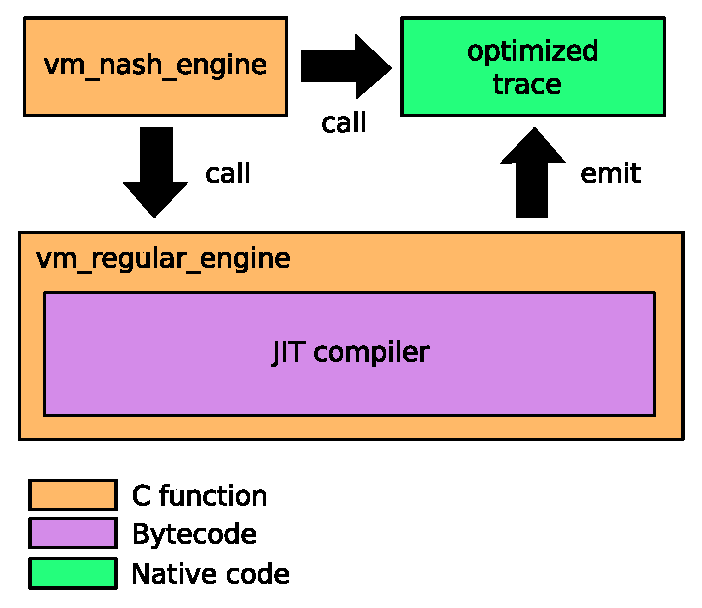
\includegraphics[width=0.4 \textwidth]{overview}
  \caption{A diagram showing software components and language its written.}
\label{fig:overview}
\end{figure}

\subsection{Nash Overview}

Nash is designed as a drop-in replacement of VM-regular, could be used when
running a script, has REPL, and could be embedded in a C program as extension
language. Figure~\hyperref[fig:overview]{\ref{fig:overview}} contains a diagram
showing which software components are written as C function, compiled bytecode,
or JIT compiled native code. C function \texttt{vm\_nash\_engine} is the
interpreter used by Nash, which does the bytecode interpretation to count loops,
record the instructions in loops, and calls compiled native code. When traces
and stack values are recorded, \texttt{vm\_nash\_engine} calls
\texttt{vm\_regular\_engine}, the C function used by VM-regular, and pass the
recorded trace and stack values. The bytecode of compiler used by
\texttt{vm\_regular\_engine} is written in Scheme. After successful compilation,
\texttt{vm\_regular\_engine} emits a native code of the input trace. The native
code is called from \texttt{vm\_nash\_engine} when the same loop was
encountered.

\begin{figure}
  \centering
  \small
\begin{verbatim}
static SCM
VM_NAME (scm_i_thread *thread, struct scm_vm *vp,
         scm_i_jmp_buf *registers, int resume)
{
  ...
  VM_DEFINE_OP (1, call, ...)
    {
      ...
      VM_NASH_CALL (old_ip);
    }
  ...
  VM_DEFINE_OP (3, tail_call ...)
    {
      ...
      VM_NASH_TAIL_CALL (old_ip);
    }
  ...
  VM_DEFINE_OP (33, br, ...)
    {
      ...
      VM_NASH_JUMP (offset);
    }
  ...
  VM_DEFINE_OP (152, uadd_immediate, ...)
    {
      ...
      NEXT (1);
    }
  ...
}
\end{verbatim}
\caption{Modified \texttt{VM\_NAME} function shown in
  Figure~\hyperref[fig:vmnameorig]{\ref{fig:vmnameorig}}.}
\label{fig:vmnamenash}
\end{figure}

\begin{figure*}
  \centering
  \small
\begin{verbatim}
7f4ddb7fc574  (uadd/immediate 0 6 1)            ; #(#x3e #x2a2 #x1 #x0 #x3e8 #x7f4ddb808660 #x3e)
7f4ddb7fc578  (vector-ref 6 5 6)                ; #(#x3f #x2a2 #x1 #x0 #x3e8 #x7f4ddb808660 #x3e)
7f4ddb7fc57c  (br-if-u64-<-scm 3 6 #t 4)        ; #(#x3f #x2a2 #x1 #x0 #x3e8 #x7f4ddb808660 #x1a)
7f4ddb7fc588  (add 1 1 6)                       ; #(#x3f #x2a2 #x1 #x0 #x3e8 #x7f4ddb808660 #x1a)
7f4ddb7fc58c  (br-if-u64-<= 4 0 #f 9)           ; #(#x3f #x2ba #x1 #x0 #x3e8 #x7f4ddb808660 #x1a)
7f4ddb7fc598  (mov 6 0)                         ; #(#x3f #x2ba #x1 #x0 #x3e8 #x7f4ddb808660 #x1a)
7f4ddb7fc59c  (br -10)                          ; #(#x3f #x2ba #x1 #x0 #x3e8 #x7f4ddb808660 #x3f)
\end{verbatim}
\caption{Bytecode instructions and stack values recorded with running
  \texttt{sample-sum}.}
\label{fig:trace}
\end{figure*}

\subsection{VM Engine For Nash}
The bytecode interpreter in Nash uses the \texttt{vm-engine.c} file, which was
used for defining vm engines as described in
Section~\hyperref[sec:background]{\ref{sec:backgroundguile}}.  The file
\texttt{vm-engine.c} is included once more with similar code to below:

\begin{verbatim}
  #define VM_NAME vm_nash_engine
  #define VM_NASH 1
  #include "vm-engine.c"
  #undef VM_NAME
\end{verbatim}

Few small modifications were made to \texttt{vm-engine.c}. Nash followed the
approach taken by RPython~\cite{bolz2009tracing} framework. Nash adds two kinds
of macros to mark interpreter, one for recording instructions, and others to
detect the loop and execute the native code. A C macro \texttt{VM\_NASH\_MERGE}
is used for recording, and three C macros \texttt{VM\_NASH\_JUMP},
\texttt{VM\_NASH\_CALL}, and \texttt{VM\_NASH\_TCALL} are used for detecting
loops and entering compiled native code.

\subsubsection{Finding Loops}

Figure~\hyperref[fig:vmnamenash]{\ref{fig:vmnamenash}} contains a snippet of
modification made to \texttt{VM\_NAME}. How \texttt{VM\_NASH\_JUMP},
\texttt{VM\_NASH\_CALL}, and \texttt{VM\_NASH\_TCALL} are used for bytecode
definitions \texttt{br}, \texttt{call}, and \texttt{tail-call} is shown.
Bytecode definitions which do not start a loop, such as
\texttt{uadd\_immediate}, are unmodified. The definition of \texttt{br} contains
\texttt{VM\_NASH\_JUMP} with a parameter \texttt{offset} at the end of
definition body. When \texttt{offset} was negative, it means a backward jump
which is detected as a loop by Nash. When \texttt{br} with negative offset was
found in interpreted bytecode, \texttt{vm\_nash\_engine} looks for a native code
with the next IP.\@

%% Sentences describing type check commented out for simplicity.
%%
%% Nash does a type check, using the types derived from values in current stack
%% contents, and the types used at the time of compilation. This type check
%% supports polymorphic behaviors in some bytecode operations, such as
%% arithmetic operations. After successful compilation, native code compiler
%% saves a Scheme object called \textit{fragment}, which contains compiled
%% native code and other information such as type information for type check.

If a native code with matching types was found, the native code is executed. If
not found, \texttt{vm\_nash\_engine} increment the counter value for the IP, and
if the counter value exceeds a threshold parameter, \texttt{vm\_nash\_engine}
starts recording. For instance, \texttt{vm\_nash\_engine} can find the loop in
\texttt{sample-sum} from the bytecode \texttt{(br~-10)} in IP $32$ of
Figure~\hyperref[fig:bytecode]{\ref{fig:bytecode}}.

Codes used internally in \texttt{VM\_NASH\_JUMP}, \texttt{VM\_NASH\_CALL}, and
\texttt{VM\_NASH\_TCALL} are mostly shared. One of the differences between these
three macros are to mark the start and end of the loop with different IP
value. Another difference is to use different strategy to decide loops as hot,
by using different values to increment loop counter. For instance,
\texttt{VM\_NASH\_JUMP} may add $2$ to the loop counter, while
\texttt{VM\_NASH\_CALL} may add $1$, which will result in a setting that
backward jumps get hot sooner than consequent calls. \texttt{VM\_NASH\_JUMP},
\texttt{VM\_NASH\_CALL}, \texttt{VM\_NASH\_TACLL} are defined as \texttt{NEXT}
when including \texttt{vm-engine.c} file for \texttt{vm\_regular\_engine} and
\texttt{vm\_debug\_engine}.

\subsubsection{Recording Instructions}

\begin{figure}
  \centering
  \small
\begin{verbatim}
# define NEXT(n)                                \
  do                                            \
    {                                           \
      ip += n;                                  \
      VM_NASH_MERGE ();                         \
      ...
      op = *ip;                                 \
      goto *jump_table[op & 0xff];              \
    }                                           \
  while (0)
\end{verbatim}
\caption{Modified definition of \texttt{NEXT}.}
\label{fig:cnext}
\end{figure}

Figure~\hyperref[fig:trace]{\ref{fig:trace}} shows dumped sample data of
recorded bytecode and stack values, and
Figure~\hyperref[fig:cnext]{\ref{fig:cnext}} shows the modified contents of
\texttt{NEXT}. When \texttt{vm\_nash\_engine} find a loop, observed bytecode and
stack values are recorded by
\texttt{VM\_NASH\_MERGE}. Figure~\hyperref[fig:cnext]{\ref{fig:cnext}} shows how
the interpretation continues with updating the value of \texttt{ip}, which is a
variable in \texttt{VM\_NAME} used for bytecode \textit{instruction
  pointer}. When the \texttt{ip} match with beginning of the loop,
\texttt{VM\_NASH\_MERGE} will stop the recording, and pass the recorded data to
JIT compiler. The recorded bytecode instructions and stack values in
Figure~\hyperref[fig:trace]{\ref{fig:trace}} were made by running
\texttt{sample-sum} with passing a length 1000 \texttt{vector} containing random
small integer numbers from \texttt{-10} to \texttt{10}. The hexadecimal numbers
in left are the absolute bytecode IP of each bytecode instruction, and the
commented out vector in each line contains \texttt{SCM} representation of the
values in the stack at the time of recording.  The first bytecode
\texttt{(uadd/immediate 0 6 1)} in Figure~\hyperref[fig:trace]{\ref{fig:trace}}
is shown at IP offset 22 in
Figure~\hyperref[fig:bytecode]{\ref{fig:bytecode}}. \texttt{vm\_nash\_engine}
continued the recording with IP offset 23, 24, 27, 28, 31. Then at IP offset 32,
the last bytecode \texttt{(br -10)} is recorded and jumped back to IP offset 22,
which is labeled as \texttt{L2} in
Figure~\hyperref[fig:bytecode]{\ref{fig:bytecode}}. The bytecode IP matched with
the IP where the recording started, \texttt{vm\_nash\_engine} stopped the
recording. \texttt{VM\_NASH\_MERGE} is defined with empty body when including
\texttt{vm-engine.c} file for \texttt{vm\_regular\_engine} and
\texttt{vm\_debug\_engine}.

%% Approach for recording of trace is different from Pycket. Pycket had a
%% problem with \textit{cyclic-path}, but Nash didn't. Might worth explaining
%% the natural-loop-first (NLF) approach taken by LuaJIT.

\begin{figure}
  \centering
  \small
\begin{verbatim}
 1  (lambda ()
 2   (let* ((_    (%snap 0))
 3          (v0   (%fref 0 #f))
 4          (v1   (%fref 1 1))
 5          (v3   (%fref 3 67108864))
 6          (v4   (%fref 4 67108864))
 7          (v5   (%fref 5 131072))
 8          (v6   (%fref 6 67108864)))
 9     (loop v0 v1 v3 v4 v5 v6)))
10  (lambda (v0 v1 v3 v4 v5 v6)
11   (let* ((v0   (%add v6 1))
12          (_    (%snap 1 v0 v1 v6))
13          (r2   (%cref v5 0))
14          (r2   (%rsh r2 8))
15          (_    (%lt v6 r2))
16          (r2   (%add v6 1))
17          (v6   (%cref v5 r2))
18          (_    (%snap 2 v0 v1 v6))
19          (_    (%typeq v6 1))
20          (_    _)
21          (r2   (%rsh v6 2))
22          (_    (%lt v3 r2))
23          (v1   (%add v1 v6))
24          (v1   (%sub v1 2))
25          (_    (%snap 3 v0 v1 v6))
26          (_    (%gt v4 v0))
27          (v6   v0))
28     (loop v0 v1 v3 v4 v5 v6)))
\end{verbatim}
\caption{IR of recorded trace in relaxed A-normal form.}
\label{fig:anf}
\end{figure}

\section{Nash Compiler}
\label{sec:compiler}

This section describes details of the JIT compiler in Nash, which is written in
Scheme. Compiled bytecode of the JIT compiler is executed by
\texttt{vm\_regular\_engine}.

\subsection{Trace To IR}
Nash compiles traces to relaxed A-normal form~\cite{flanagan1993essence}
internal representation (IR) before assigning registers and assembling to native
code. Figure~\hyperref[fig:anf]{\ref{fig:anf}} shows IR of primitive operations
compiled from the recorded trace in
Figure~\hyperref[fig:trace]{\ref{fig:trace}}. The IR primitives contains two
\texttt{lambda} terms, the first block is for prologue, and the second block is
for loop body. The IR uses \texttt{let*} instead of \texttt{let} to express the
sequence of computation. Each primitive operation takes two arguments, except
for \texttt{\%snap} operation. Primitive operations updating the value of
variable, such as \texttt{\%add}, has a variable on the left side of expression,
which its value is updated by the corresponding operation. Primitive operations
without variable update contains symbol \texttt{\_} at the left side of
expression. The variables starting with the letter \texttt{v} indicates that the
variable is loaded from current stack. The variables starting with the letter
\texttt{r} indicates that the variable is for temporal use only.

\subsubsection{Snapshot}

Between recorded bytecode operation, \texttt{\%snap} expressions are inserted to
make \textit{snapshot} data. Snapshot contains various information to recover
the state of \texttt{vm\_nash\_engine} when native code passed the control back,
including the local indices to store variables, and a bytecode IP where the
interpretation of bytecode program continue. The expression \texttt{\%snap}
takes variable number of arguments: the first argument is a \textit{snapshot
  ID}, which is a unique integer number to identify the snapshot in single
trace. The rest of the arguments are local variables to be stored to stack used
by \texttt{vm\_nash\_engine}. In Figure~\hyperref[fig:anf]{\ref{fig:anf}}, Nash
inserted \texttt{\%snap} expression before the primitive operations
\texttt{\%lt}, \texttt{\%typeq}, and \texttt{\%gt}, which act as guard. The
primitives \texttt{\%lt} and \texttt{\%gt} does arithmetic less-than and
greater-than comparisons, respectively, and the primitive \texttt{\%typeq} does
type check with given variable and type. When the result of guard differed from
the result observed at the time of JIT compilation, native code execute the
recovering steps to setup the state in \texttt{vm\_nash\_engine}, and input
program continues with bytecode.


\subsubsection{Prologue section}

The prologue section, the first \texttt{lambda} block shown in
Figure~\hyperref[fig:anf]{\ref{fig:anf}}, loads initial values from the stack
with \texttt{\%fref} primitive. The first argument number passed to
\texttt{\%fref} is a local index offset, the second argument is an integer to
represent type of expected local in the stack. For instance, the value
\texttt{1} is for \texttt{fixnum}, which means small integer value in Scheme,
\texttt{131072} is used for vector object, \texttt{67108864} is for
\texttt{u64}, which is a non-SCM unsigned 64 bit integer value, and so on.

Type information are specified from bytecode operation, or from the stack values
recorded alongside with bytecode instructions. The tc3 tag, described in
Section~\ref{sec:scmdatatype}, of each value is observed and type check for the
locals are added when necessary. For instance, in the line containing
\texttt{(add~1~1~6)} in Figure \hyperref[fig:trace]{\ref{fig:trace}}, the second
element in the stack is \texttt{\#x2a2}, which is \texttt{1010100010} in
binary. Nash could decide this value as a small integer, since it has tc3 tag
\texttt{010} shown in Table~\hyperref[tab:tags]{\ref{tab:tags}}.

The value \texttt{\#f} in \texttt{\%fref} primitive means that there is no need
for type check, for instance, the local is overwritten without
referencing. Indeed, the variable \texttt{v0}, which hold local \texttt{0} in
above example is immediately overwritten by result of \texttt{\%add} primitive
in loop body. This local is not needed to be loaded from stack, though such
dead-code eliminations are not yet implemented.

\subsubsection{Loop body section}

The loop body section, the second \texttt{lambda} block in Figure
\hyperref[fig:anf]{\ref{fig:anf}}, is compiled by translating each recorded
bytecode instruction sequentially.

\paragraph{uadd/immediate} The first primitive operation contains
\texttt{\%add}, which does arithmetic addition with variable \texttt{v6} and
constant value $1$. The result of addition overwrites variable \texttt{v0}.

\paragraph{vector-ref} Then a snapshot 1 is inserted, and
the primitive operations for \texttt{vector-ref} follows. The primitive
operations contain vector index range check, by comparing the length of vector
with the index value passed to \texttt{vector-ref} procedure. For Scheme
\texttt{vector} object, Guile uses the first one word to store a tc7 tag and the
length of the vector. The length is left shifted for 8 bits so that tc7 tag and
the length could fit in single word. Actual vector elements are stored from the
memory address of the SCM object plus one word. The primitive operation
\texttt{\%cref} in line 13 loads a value from Scheme heap object with given
offset, then store the loaded value to temporary register \texttt{r2}. The
\texttt{r2} is passed to \texttt{\%rsh} in line 14, which does arithmetic right
shift for 8 bits, and overwrite the value of \texttt{r2} itself. Now the
variable \texttt{r2} contains the reproduced vector length, and compared with
\texttt{v6}, which is the variable holding local 6, which is the index value
used in \texttt{vector-ref} bytecode instruction of recorded trace. Line 16 adds
$1$ to \texttt{v6} get offset of vector element. Line 17 does another
\texttt{\%cref} to load the vector element, and overwrites the value of
\texttt{v6}.

\paragraph{br-if-u64-\texttt{<}-scm} Line 18 contains a snapshot used by next
primitive operation \texttt{\%typeq}, which does a type check of \texttt{v6}
with \texttt{fixnum}, the type representing small integers. The variable
\texttt{v6} is the value loaded from \texttt{vector}, which was observed as
\texttt{fixnum} at the time of JIT compilation. Line 20 shows empty value
assigned to empty value, which was a line containing a \texttt{\%snap}
operation. Nash has optimized away the snapshot, since the bytecode IP
destination in snapshot data was identical to the previous snapshot. Nash does
few on-the-fly optimizations like this use of cached snapshot, such as constant
folding.  Variable \texttt{v6} is right shifted for 2 bits to move away the tc3
tag of \texttt{fixnum}, and the result is stored to variable \texttt{r2} in line
21, to compare with variable \texttt{v3} shown in line 22. Bytecode instruction
\texttt{br-if-u64-<-scm} takes \texttt{u64} type as first argument, SCM type as
second argument, and compares the two. The type of variable \texttt{v3} is
determined at compile time as \texttt{u64}, no type check is done.

\paragraph{add} Line 23 adds two \texttt{fixnum} values in \texttt{v1} and
\texttt{v6}, and overwrites the contents of \texttt{v1}. The \texttt{\%sub}
primitive in line 24 moves away the extra tc2 bits added by \texttt{\%add}
primitive.

\paragraph{br-if-u64-\texttt{<}=} Line 25 inserts another snapshot. Then in line
26, two 64 bit unsigned values in \texttt{v4} and \texttt{v0} are
compared. Types of variables are determined from the bytecode.

\paragraph{mov} Line 27 simply does a move, and overwrites the contents of
\texttt{v6} with \texttt{v0}.

\paragraph{br} Then the IR shows a call to \texttt{loop}, which tells that the
computation jumps to the beginning of loop body section. Loop body of native
code exit when any of the guards failed.  For instance, when the result returned
by \texttt{(\%gt~v4~v0)} differed from the result observed at the time of JIT
compilation, native code will pass the control back to
\texttt{vm\_nash\_engine}, recover the interpreter state by using snapshot data
from \texttt{(\%snap~3~v0~v1~v6)} and the bytecode interpretation of input
program will continue from bytecode IP \texttt{7f4ddb7fc5b0}, which is the jump
destination of \texttt{(br-if-u64-<=~4~0~\#f~9)} in recorded trace.
\footnote{ \texttt{7f4ddb7fc5b0 = 7f4ddb7fc8c + (9 * 4)}.  \texttt{7f4ddb7fc8c}
  is the absolute bytecode IP of \texttt{(br-if-u64-<= 4 0 \#f 9)} shown in
  recorded trace, $9$ is the offset argument passed to \texttt{br-if-u64-<=},
  and $4$ is the size of one byte}


\begin{figure}
  \centering
  \small
\begin{verbatim}
----     [snap  0] ()
0001     (%fref    r14 +0 ---)
0002     (%fref    r15 +1 fixn)
0003     (%fref    r9 +3 u64)
0004     (%fref    r8 +4 u64)
0005     (%fref    rcx +5 vect)
0006     (%fref    rdx +6 u64)
==== loop:
0007     (%add     r14 rdx +1)
----     [snap  1] ((0 u64) (1 fixn) (6 u64))
0009     (%cref    r11 rcx +0)
0010     (%rsh     r11 r11 +8)
0011   > (%lt      rdx r11)
0012     (%add     r11 rdx +1)
0013     (%cref    rdx rcx r11)
----     [snap  2] ((0 u64) (1 fixn) (6 scm))
0015   > (%typeq   rdx fixn)
0016     (%rsh     r11 rdx +2)
0017   > (%lt      r9 r11)
0018     (%add     r15 r15 rdx)
0019     (%sub     r15 r15 +2)
----     [snap  3] ((0 u64) (1 fixn) (6 scm))
0021   > (%gt      r8 r14)
0022     (%move    rdx r14)
==== ->loop
\end{verbatim}
\caption{Primitive operation of recorded trace under x86-64
  architecture. Slightly modified from dumped output for displaying purpose.}
\label{fig:primops}
\end{figure}

\begin{figure}
  \centering
  \small
\begin{verbatim}
0x00f9405b mov    rax,QWORD PTR [rbx]
0x00f9405e mov    r14,rax
0x00f94061 mov    rax,QWORD PTR [rbx+0x8]
0x00f94065 mov    r15,rax
0x00f94068 mov    rax,QWORD PTR [rbx+0x18]
0x00f9406c mov    r9,rax
0x00f9406f mov    rax,QWORD PTR [rbx+0x20]
0x00f94073 mov    r8,rax
0x00f94076 mov    rax,QWORD PTR [rbx+0x28]
0x00f9407a mov    rcx,rax
0x00f9407d mov    rax,QWORD PTR [rbx+0x30]
0x00f94081 mov    rdx,rax
0x00f94084 nop    DWORD PTR [rax+0x0]
loop:
0x00f94088 lea    r14,[rdx+0x1]
0x00f9408c mov    r11,QWORD PTR [rcx]
0x00f9408f sar    r11,0x8
0x00f94093 cmp    rdx,r11
0x00f94096 jge    0x00fa1028    ->1
0x00f9409c lea    r11,[rdx+0x1]
0x00f940a0 lea    rax,[r11*8+0x0]
0x00f940a8 mov    rdx,QWORD PTR [rax+rcx*1]
0x00f940ac test   rdx,0x2
0x00f940b3 je     0x00fa1030    ->2
0x00f940b9 mov    r11,rdx
0x00f940bc sar    r11,0x2
0x00f940c0 cmp    r9,r11
0x00f940c3 jge    0x00fa1030    ->2
0x00f940c9 add    r15,rdx
0x00f940cc sub    r15,0x2
0x00f940d0 cmp    r8,r14
0x00f940d3 jle    0x00fa1038    ->3
0x00f940d9 mov    rdx,r14
0x00f940dc jmp    0x00f94088    ->loop
0x00f940e1 nop    DWORD PTR [rax+0x0]
\end{verbatim}
\caption{Native code of compiled primitive operations under x86-64
  architecture.}
\label{fig:ncode}
\end{figure}

\subsection{IR To Native Code}
Figure~\hyperref[fig:primops]{\ref{fig:primops}} shows IR after register
assignment. The numbers in left of each line, which are omitted for snapshot
data, tells primitive operation number. The variables for primitive operations
in Figure~\hyperref[fig:primops]{\ref{fig:primops}} are using register names in
x86-64 architecture. Nash uses a module which defines architecture specific
register variables. At the time of writing, x86-64 implementation is the only
one which exist.

Nash uses GNU lightning as an assembler backend\cite{}. GNU lightning is a JIT
compilation library, which runs under various architectures including aarch64,
alpha, arm, ia64, mips, powerpc, s390, sparc, and x86. Nash contains a thin C
wrapper which binds SCM type to the types understood by GNU lightning. The
resulting bindings are called from Scheme code under
\texttt{vm\_regular\_engine} just like other Scheme procedures defined in
C.

Figure~\hyperref[fig:ncode]{\ref{fig:ncode}} shows dumped native code of
primitive operations shown in Figure~\hyperref[fig:primops]{\ref{fig:primops}}
under x86-64 architecture. The native code contains a mark to show the beginning
of loop body with \texttt{loop:}, and corresponding snapshot ID number for jump
instructions.

Native code compiled in Nash contains debug symbol to interact with JIT
compilation interface in GDB, a well-known open-source debugger. This debugging
support is turned off by default, turned on by passing command line option when
invoking \texttt{guile} executable.
\footnote{Other than debug symbol, Nash contains a command line option to dump
  intermediate data of compilation. Contents of
  Figure~\hyperref[fig:anf]{\ref{fig:anf}},
  \hyperref[fig:primops]{\ref{fig:primops}}, and
  \hyperref[fig:ncode]{\ref{fig:ncode}} are obtained from the dumped output.}

\section{Evaluation}
\label{sec:evaluation}

\begin{figure}
  \centering
  \includegraphics[angle=270,origin=c,width=0.5 \textwidth]{bench}
  \caption{Relative total time of benchmarks and geometric mean normalized to
    Guile VM-regular. Smaller is better.}
\label{fig:bench}
\end{figure}

\subsection{Settings}

Performance of Nash is evaluated with modified cross platform benchmark suite
from Pycket project. The source code of the benchmarks originate from Larceny
and Gambit project. Slight modifications were done to the Pycket version for
evaluating Nash. Benchmarks \texttt{ntakl} and \texttt{quicksort} were enabled,
and iteration counts for \texttt{ctak}, \texttt{fft}, \texttt{pnpoly},
\texttt{fibc}, and \texttt{ray} are decreased, which were taking long execution
time in Guile's VM-regular. The modified benchmark suite contains 56
programs. The benchmark results were taken under a machine with Intel Core-i5
3427-U and 8GB of memory, running Arch Linux, Linux kernel 4.5.4. The Scheme
implementations and its versions used are Guile VM-regular version 2.1.2, Racket
version 6.5, and Pycket git revision 5f98bfe (with RPython hg revision
83529:2179c). Total elapsed time of each program including JIT warm up time was
measured.

\begin{table}
  \centering
  \begin{tabular}{rccc}
    \toprule
    Benchmark name & Nash & Racket & Pycket\\
    \midrule
    sumfp & 0.025 & 0.127 & 0.015 \\
    mbrot & 0.036 & 0.122 & 0.018 \\
    sum & 0.075 & 0.373 & 0.088 \\
    \midrule
    ctak & 1.036 & 1.050 & 0.091 \\
    fibc & 1.434 & 1.116 & 0.095 \\
    \midrule
    paraffins & 1.178 & 0.725 & 1.500 \\
    parsing & 1.985 & 0.149 & 0.154 \\
    dynamic & 4.671 & 0.549 & 2.043 \\
    \midrule
    Geometric mean & 0.416 & 0.310 & 0.235 \\
    \bottomrule
  \end{tabular}
  \caption{Selected benchmark results and geometric mean in
    Figure~\hyperref[fig:bench]{\ref{fig:bench}} shown in numbers.}
\label{tab:bench}
\end{table}

\subsection{Results}

Figure~\ref{fig:bench} shows relative total time of each benchmark and geometric
mean normalized to Guile's VM-regular. The range of the plot in the figure is
limited from 0 to 2 for displaying
purpose. Table~\hyperref[tab:bench]{\ref{tab:bench}} contains selected benchmark
results and geometric mean shown in numbers.  Geometric means of 56 benchmarks
shows that Nash runs approximately $2.4\times$ \textit{faster} than VM-regular,
$1.3\times$ \textit{slower} than Racket, and $1.8\times$ \textit{slower} than
Pycket.  Some of the benchmarks have shown significant performance improvement
in Nash compared to VM-regular. Benchmark \texttt{sumfp} and \texttt{mbrot}
contain tight loop with Scheme \texttt{flonum}. Nash runs \texttt{sumfp}
$40\times$ faster, and \texttt{mbrot} $25\times$ faster than VM-regular. The
results of \texttt{sumfp} and \texttt{mbrot} are about $5\times$ and $3.3\times$
faster than Racket, respectively. However, both benchmarks still run slower than
Pycket.  Some of the benchmarks performed worse than Guile's
VM-regular. Benchmark \texttt{parsing} and \texttt{dynamic} contain program to
parse a Scheme source code. These programs include lots of branching
conditions. The \texttt{parsing} and \texttt{dynamic} performed about $2\times$
and $5\times$ slower than VM-regular, respectively.

\section{Related Work}
\label{sec:related}
Implementation of Nash was inspired from pioneers in tracing JIT field. Nash
does type checks in VM interpreter before running compiled native code, which
was done TraceMonkey~\cite{gal2009trace} with similar design.

Use of A-normal form~\cite{flanagan1993essence} was inspired from
Pycket~\cite{bauman2015pycket}. Though Pycket expand the source code and
generates JSON data, and parses it to AST for execution.  Both Nash and Pycket
use tracing JIT in its implementation. Both performed well with benchmarks
containing tight loop, such as \texttt{sumfp}, \texttt{sum}, and
\texttt{sumloop}. Pycket performed better than Nash, except for
\texttt{sum}. From Table~\hyperref[tab:bench]{\ref{tab:bench}}, Pycket performed
well with benchmark containing extensive use of \texttt{call/cc}, such as
\texttt{fibc} and \texttt{ctak}. Nash implements \texttt{call/cc} with C stack,
to keep compatibility with C interface of VM-regular, which did not led to
performance improvement. Both performed bad in benchmarks containing lots of
condition branches, such as \texttt{paraffins} and \texttt{dynamic}. Nash
performed bad in \texttt{parsing} benchmark also, but the performance of
\texttt{parsing} in Pycket was close to Racket.

Design of snapshot was inspired from LuaJIT~\cite{pall2016luajit}. LuaJIT uses
more sophisticated approach and compresses snapshot data. LuaJIT used
NaN-tagging~\cite{pall2009ip}, which enables efficient handling of unboxed
floating point numbers. Guile once had an attempt to use
NaN-tagging~\cite{wingo2011value}, though the attempt wasn't merged to Guile
source code, due to supporting conservative garbage collector under 32 bit
architectures.

\section{Future Work}
\label{sec:future}

Nash is still an experimental implementation, still has a lot of space for
improvement. Some of the possibilities for future works follows.

\paragraph{Support more bytecode instructions} Nash still have bytecode
instructions which are not implemented at all, such as \texttt{prompt} and
\texttt{abort} used for delimited continuation, or partially implemented, such
as arithmetic operations. Arithmetic operations for multi-precision numbers and
complex numbers are not yet implemented. When JIT compiler encountered
unsupported bytecode, the compilation will break and control of the input
program is passed back to \texttt{vm\_nash\_engine}.

\paragraph{Detect more loops} Nash detects loops with backward jump,
tail-calls, and consequent calls for non-tail-call recursion
(\textit{down-recursion}\footnote{Consequent calls to procedure are called as
  down-recursion in Nash, because Guile's stack grows down}), though not with
consequent returns resulted from non-tail-call recursions
(\textit{up-recursion}). Nash does not detect \textit{looping side traces}. Side
trace start from frequently taken exit in native code. Side traces are usually
patched to existing trace when \texttt{vm\_nash\_engine} encountered beginning
bytecode IP of existing trace. In looping side trace, bytecode instructions loop
inside the side trace, instead of patched back.

\paragraph{Optimize IR} Nash does only a few IR level optimizations.
More optimizations could be done, such as dead-code elimination, escape
analysis, and so on. Also, Nash currently uses naive method to assign
registers. More sophisticated method such as Linear-Scan register
allocation~\cite{poletto1999linear} could be used.

\paragraph{Blacklist} Benchmarks such as \texttt{parsing} and
\texttt{dynamic} were slower than Guile VM-regular. Programs containing large
number of branching conditions need some treatments to perform well under
tracing JIT.\@ One approach is to limit the JIT compilation when branching
exceed certain threshold. These thresholds mechanism are sometime called
\textit{blacklisting} of trace. Nash could take more sophisticated approach to
blacklist unwanted traces.

\section{Conclusion}
\label{sec:conclusion}
This paper has shown how Nash is designed. Nash reused existing bytecode
interpreter in Guile, turned it to a trace recording interpreter with small
modifications. Nash coexist with current VM, which is used for JIT compiler
written in Scheme. Existing bytecode compiled by Guile are traced, recorded and
compiled to native code. Resulting native codes have shown significant
performance improvement in several of the benchmarks. Performance comparison
between Nash, Guile's VM-regular and other Scheme implementations were
done. Benchmarks have shown close performance with native code compilers such as
Racket and Pycket when assumptions for tracing JIT were met.

%% \appendix
%% \section{Appendix: title}
%% This is the text of the appendix, if you need one.

%% \acks{} Acknowledgments, if needed.
\acks{} Nash exist because of the hard works done for GNU Guile, by many open
source developers.

% We recommend abbrvnat bibliography style.

\bibliographystyle{abbrvnat}

% The bibliography should be embedded for final submission.

%% \begin{thebibliography}{}
%% \softraggedright{}
%% ...
%% \end{thebibliography}

% Using .bib file at the moment.
\bibliography{guile-tjit}

\end{document}

%%  LocalWords:  AOT Pycket ANF TinyScheme Gauch Ypsilon SCM disassembler tc
%%  LocalWords:  typedef Immediates immediates LuaJIT Pypy Lua Rpython fixnum
%%  LocalWords:  RPython backend sparc powerpc mips aarch ia TraceMonkey JSON
%%  LocalWords:  AST unboxed NaN bytecode JIT TCALL untagging
